\documentclass[10pt,letterpaper]{article}
% ------------------------------------------------------------------
%  Reporte: Pintor Evolutivo (AG para replicar imagenes con pinceladas)
%  Compilar en Overleaf con pdfLaTeX. Las cifras vienen de numeros.tex,
%  generado por generar_figuras.py a partir de la carpeta resultados/.
% ------------------------------------------------------------------
\usepackage[utf8]{inputenc}
\usepackage[T1]{fontenc}
\usepackage[spanish,es-tabla,es-nodecimaldot]{babel}
\usepackage{lmodern}
\usepackage[margin=2cm]{geometry}
\usepackage{amsmath,amssymb}
\usepackage{graphicx}
\usepackage{booktabs}
\usepackage{caption}
\captionsetup{font=small,labelfont=bf}
\usepackage{algorithm}
\usepackage{algpseudocode}
\usepackage[hidelinks]{hyperref}
\usepackage{xcolor}
\setlength{\parskip}{0.25em}
\renewcommand{\algorithmicrequire}{\textbf{Entrada:}}
\renewcommand{\algorithmicensure}{\textbf{Salida:}}
\floatname{algorithm}{Algoritmo}

% Generado automaticamente por generar_figuras.py: no editar a mano
\newcommand{\vgMSE}{0.00418}
\newcommand{\vgPSNR}{23.79}
\newcommand{\vgSSIM}{0.732}
\newcommand{\vgTiempo}{9.9}
\newcommand{\vgEtapas}{21749}
\newcommand{\vgRech}{1749}
\newcommand{\vgEval}{4.52}
\newcommand{\moMSE}{0.00074}
\newcommand{\moPSNR}{31.30}
\newcommand{\moSSIM}{0.887}
\newcommand{\moTiempo}{11.1}
\newcommand{\moEtapas}{25656}
\newcommand{\moRech}{5656}
\newcommand{\moEval}{5.34}
\newcommand{\agMSE}{0.00462}
\newcommand{\agSD}{0.00002}
\newcommand{\alMSE}{0.00517}
\newcommand{\alSD}{0.00002}
\newcommand{\agPSNR}{23.36}
\newcommand{\alPSNR}{22.87}
\newcommand{\agSSIM}{0.700}
\newcommand{\alSSIM}{0.657}
\newcommand{\agT}{74}
\newcommand{\alT}{57}
\newcommand{\agEval}{626}
\newcommand{\alEval}{624}
\newcommand{\mejora}{10.7}
\newcommand{\ebMSE}{0.00496}
\newcommand{\ebPSNR}{23.04}
\newcommand{\ebSSIM}{0.667}
\newcommand{\ebT}{73}
\newcommand{\ebEval}{820}
\newcommand{\kTresMSE}{0.00760}
\newcommand{\kTresT}{59}
\newcommand{\kUnoMSE}{0.00462}
\newcommand{\kUnoT}{74}
\newcommand{\lamCeroMSE}{0.00635}
\newcommand{\lamCeroDes}{0.064}
\newcommand{\lamCeroSSIM}{0.654}
\newcommand{\lamMedMSE}{0.00645}
\newcommand{\lamMedDes}{0.017}
\newcommand{\lamMedSSIM}{0.651}
\newcommand{\lamAltoMSE}{0.00662}
\newcommand{\lamAltoDes}{0.004}
\newcommand{\lamAltoSSIM}{0.645}


\title{\vspace{-1.2cm}\textbf{Pintor evolutivo: replicación de imágenes con pinceladas\\ al estilo de Van Gogh y Monet mediante un algoritmo genético}}
\author{Angie \textit{[apellidos]} \and Leo \textit{[apellidos]} \and \textit{[tercer integrante]}\\[2pt]
\small Maestría --- Optimización \quad \small\textit{[Institución]}}
\date{\small Noviembre de 2026}

\begin{document}
\maketitle
\vspace{-0.6cm}

\begin{abstract}
\noindent Se presenta un algoritmo genético (AG) de codificación real que reproduce una fotografía mediante miles de pinceladas parametrizadas: posición, ángulo, largo, grosor, transparencia, color y curvatura. El problema completo, de decenas de miles de variables, se descompone en una secuencia de subproblemas de 10 variables. En cada etapa un AG con selección por torneo, cruza BLX-$\alpha$, mutación gaussiana y elitismo busca la pincelada que más reduce el error cuadrático medio (MSE) entre el lienzo y la imagen objetivo. El estilo se incorpora en tres niveles: la forma de las pinceladas, un objetivo estilizado y un término de alineación con el campo de flujo de la imagen en la función de aptitud. Con 20{,}000 pinceladas se obtiene un PSNR de \vgPSNR~dB (Van Gogh) y \moPSNR~dB (Monet). Con el mismo número de evaluaciones de aptitud, el AG reduce el MSE un \mejora\,\% respecto a una búsqueda aleatoria guiada.
\end{abstract}

% ==================================================================
\section{Introducción}
La pintura por computadora basada en trazos (\emph{stroke-based rendering}) busca imitar el proceso de un pintor: colocar trazos discretos sobre un lienzo hasta aproximar una imagen \cite{haeberli,hertzmann}. Formulado como problema de optimización, se trata de encontrar el conjunto de pinceladas que minimiza la diferencia entre el lienzo y la imagen de referencia. El espacio de búsqueda es enorme, continuo, no diferenciable (los trazos se rasterizan) y multimodal, lo que lo vuelve un buen caso para la computación evolutiva \cite{engelbrecht}.

El objetivo del proyecto es construir un AG que, dada una imagen de entrada, genere una versión pintada con el estilo de Vincent van Gogh (trazos largos, empastados y orientados siguiendo las formas) o de Claude Monet (toques cortos, semitransparentes y de color quebrado). El trabajo integra dos avances previos del equipo: un diseño orientado a objetos de pinceladas \texttt{line}/\texttt{arc} con un generador aleatorio, y un AG de codificación real con torneo, BLX-$\alpha$ y mutación gaussiana.

% ==================================================================
\section{Marco teórico}
Un algoritmo evolutivo mantiene una población de soluciones candidatas (cromosomas) que se modifican mediante \emph{selección}, \emph{recombinación} y \emph{mutación}, guiadas por una función de aptitud \cite[cap.~8]{engelbrecht}. En los AG de codificación real \cite[cap.~9]{engelbrecht} cada gen es un número real, lo que evita la discretización binaria y permite operadores aritméticos:
\begin{itemize}\setlength\itemsep{0em}
\item \textbf{Selección por torneo:} se eligen $k$ individuos al azar y gana el de mejor aptitud. La presión selectiva se controla con $k$.
\item \textbf{Cruza BLX-$\alpha$} \cite{blx}: para padres $x,y$ y $d=|x-y|$, cada gen del hijo se muestrea de $U[\min(x,y)-\alpha d,\ \max(x,y)+\alpha d]$. Con $\alpha>0$ se puede explorar fuera del segmento entre los padres.
\item \textbf{Mutación gaussiana:} $x' = x + \mathcal{N}(0,\sigma^2)$ con probabilidad $p_m$ por gen. Reducir $\sigma$ con las generaciones hace pasar de exploración a explotación.
\item \textbf{Elitismo:} el mejor individuo pasa sin cambios a la siguiente generación, lo que garantiza que la mejor aptitud no empeore.
\end{itemize}

% ==================================================================
\section{Formulación del problema}
Sea $O\in[0,255]^{H\times W\times 3}$ la imagen objetivo y $\mathcal{R}(s_1,\dots,s_n)$ el lienzo que resulta de pintar las pinceladas $s_1,\dots,s_n$ en orden, con mezcla alfa: $L \leftarrow L(1-a)+c\,a$. Cada pincelada es un vector $s\in[0,1]^{10}$:
\[
s = (x,\ y,\ \theta,\ \ell,\ g,\ \alpha,\ r,\ v,\ b,\ \kappa),
\]
que se decodifica a centro en píxeles, ángulo $\theta\pi\in[0,\pi)$, largo $\ell$ relativo a la escala de la etapa, grosor mediante la razón largo/grosor del estilo, opacidad, color RGB y curvatura. Si $|\kappa|$ es pequeña la pincelada es una recta (\texttt{line}); si no, es un arco de circunferencia (\texttt{arc}). El problema global es
\[
\min_{s_1,\dots,s_n\in[0,1]^{10}}\ \frac{1}{3\cdot255^2\,HW}\sum_{p}\big\lVert \mathcal{R}(s_1,\dots,s_n)_p - O_p\big\rVert^2 ,
\]
con $10n$ variables, es decir $2\times10^5$ para $n=20{,}000$. Para hacerlo tratable se \textbf{descompone secuencialmente}: el lienzo actual $L_{t}$ actúa como memoria y en la etapa $t$ se resuelve solo
\begin{equation}
\min_{s\in[0,1]^{10}} f(s)= \underbrace{\frac{\lVert \mathcal{R}(L_t,s)-O\rVert^2}{3\cdot255^2\,HW}}_{\text{MSE}}
+\lambda_{\phi}\,\frac{A(s)\,w(x,y)\,\sin^2\!\big(\theta-\phi(x,y)\big)}{HW}
+\lambda_h\,(1-\text{cobertura}),
\label{eq:fitness}
\end{equation}
donde $A(s)$ es el área del trazo, $\phi$ es el \textbf{campo de flujo} (perpendicular al gradiente, obtenido del tensor de estructura) y $w=0.25+0.75\cdot$coherencia pondera la penalización según qué tan definida está la dirección local (Fig.~\ref{fig:flujo}). El segundo término codifica el rasgo de Van Gogh de orientar los trazos siguiendo las formas. El tercero recupera el término de cobertura (\emph{hedge}) del diseño original del equipo; en este trabajo $\lambda_h=0$, porque el MSE se mide sobre toda la imagen y eso ya castiga las zonas sin pintar. Las restricciones de caja se mantienen con reparación por recorte (y módulo~1 para el ángulo, que es circular).

\begin{figure}[t]
\centering
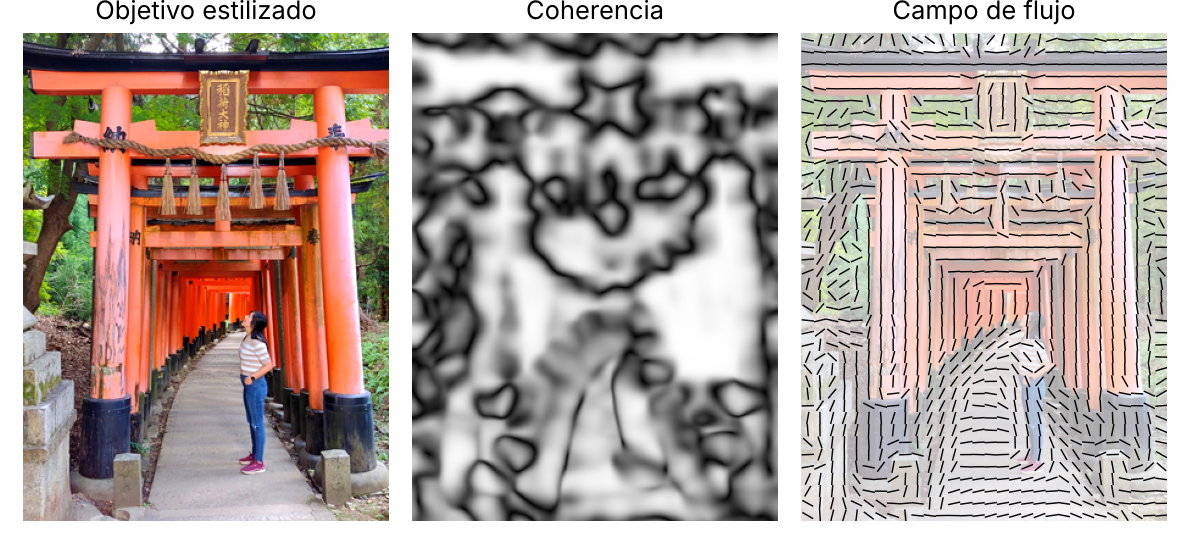
\includegraphics[width=0.78\linewidth]{figuras/flujo.png}
\vspace{-0.3cm}
\caption{Objetivo estilizado para Van Gogh (saturación $\times$1.45), coherencia del tensor de estructura y campo de flujo $\phi$, usado para inicializar y penalizar el ángulo de las pinceladas.}
\label{fig:flujo}
\vspace{-0.3cm}
\end{figure}

% ==================================================================
\section{Algoritmo propuesto}
\begin{algorithm}[t]
\caption{Pintor evolutivo (AG por etapas, de lo grueso a lo fino)}
\label{alg:pintor}
\small
\begin{algorithmic}[1]
\Require imagen $O$, estilo, total de pinceladas $n$, población $P{=}16$, generaciones $G{=}12$
\State $O \gets$ estilizar$(O)$;\quad $(\phi,\text{coh})\gets$ tensor de estructura$(O)$;\quad $L\gets$ color promedio de $O$
\While{pinceladas $< n$}
  \State $\ell_t \gets W\,\ell_{ini}(\ell_{fin}/\ell_{ini})^{(\text{pinceladas}/n)^{\gamma}}$ \Comment{escala de la etapa}
  \State foco $\sim$ error local suavizado de $L$ \Comment{se pinta donde más falta}
  \State $\mathcal{P}\gets P$ pinceladas cerca del foco, con color de $O$ y ángulo de $\phi$ \Comment{inicialización heurística}
  \For{$g=1..G$}
    \State $\sigma\gets\sigma_0(1-0.8\,g/G)$;\quad $\mathcal{P}'\gets\{\text{mejor}(\mathcal{P})\}$ \Comment{elitismo}
    \While{$|\mathcal{P}'|<P$}
       \State $p_1,p_2\gets$ torneo$_3(\mathcal{P})$;\quad $h\gets$ BLX-$\alpha(p_1,p_2)$ con prob.\ $p_c$
       \State $\mathcal{P}'\gets\mathcal{P}'\cup\{$mutación gaussiana$(h,\sigma)\}$
    \EndWhile
    \State $\mathcal{P}\gets\mathcal{P}'$; evaluar $f$ (Ec.~\ref{eq:fitness}) solo en la caja envolvente de cada trazo
  \EndFor
  \If{$f(\text{mejor})<f(L)$} pintar mejor en $L$ (y en el lienzo de alta resolución) \Else\ rechazar etapa \EndIf
\EndWhile
\end{algorithmic}
\end{algorithm}

El Algoritmo~\ref{alg:pintor} resume el método. Las decisiones de diseño principales son:

\textbf{Evaluación incremental.} El lienzo guarda un mapa de error por píxel. Evaluar una pincelada solo requiere recalcular el error dentro de su caja envolvente, $\Delta E = E_{\text{nuevo}}(\text{caja})-E_{\text{viejo}}(\text{caja})$, lo que es exacto y varios órdenes de magnitud más barato que medir toda la imagen. Si un cromosoma tiene $K>1$ pinceladas, se pinta, se mide y se deshace con una pila.

\textbf{Inicialización heurística y focos guiados por error.} Cada etapa sortea un foco con probabilidad proporcional al error local. La población inicial se coloca alrededor del foco, con el color de la imagen en esa posición y el ángulo del flujo, de modo que el AG parte de soluciones razonables y se dedica a refinarlas.

\textbf{Operadores.} Torneo ($k=3$), BLX-$\alpha$ ($\alpha=0.3$, $p_c=0.8$) con el ángulo \emph{desenrollado} antes de mezclar, porque es circular. La mutación es gaussiana ($p_m=0.25$, $\sigma_0=0.12$) con el paso espacial proporcional al tamaño del trazo, y se aplica elitismo. Una etapa solo se acepta si mejora la aptitud del lienzo.

\textbf{De lo grueso a lo fino.} El largo de las pinceladas decrece geométricamente, como en la pintura por capas \cite{hertzmann}. Como los trazos son vectoriales, el AG trabaja a $400\times533$\,px y el resultado se vuelve a dibujar a $1200\times1600$\,px, con antialiasing y textura de cerdas.

\textbf{Estilos.} El Cuadro~\ref{tab:estilos} resume los parámetros. Van Gogh satura y contrasta el objetivo y usa trazos largos, opacos y curvos alineados al flujo ($\lambda_\phi=0.04$). Monet suaviza el objetivo y usa toques cortos, anchos y semitransparentes con orientación libre ($\lambda_\phi=0$).

\begin{table}[h]
\centering\small
\caption{Parámetros de estilo (largo como fracción del ancho $W$).}
\label{tab:estilos}
\begin{tabular}{lcc}
\toprule
Parámetro & Van Gogh & Monet\\
\midrule
Objetivo: saturación / contraste / suavizado & 1.45 / 1.12 / 0 & 1.20 / 0.92 / 1.0\\
Largo inicial $\to$ final ($\ell_{ini}\to\ell_{fin}$) & $0.16\to0.018$ & $0.10\to0.02$\\
Razón largo/grosor & 2.6--4.5 & 1.3--2.2\\
Opacidad $\alpha$ & 0.80--1.00 & 0.45--0.85\\
Curvatura máx.\ / prob.\ inicial de arco & 1.4 rad / 0.50 & 0.5 rad / 0.15\\
Ángulo inicial según el flujo / $\lambda_\phi$ & 100\,\% / 0.04 & 25\,\% / 0\\
\bottomrule
\end{tabular}
\end{table}

% ==================================================================
\section{Experimentos y resultados}
Todas las corridas usan la fotografía de la Fig.~\ref{fig:final} (izquierda) y se ejecutaron en un núcleo de CPU por corrida, con Python 3, NumPy y Pillow.

\textbf{Corridas finales.} Con 20{,}000 pinceladas, Van Gogh alcanzó MSE $=\vgMSE$, PSNR $=\vgPSNR$~dB y SSIM $=\vgSSIM$ en \vgTiempo~min (\vgEtapas~etapas, \vgEval~millones de evaluaciones de aptitud). Monet alcanzó MSE $=\moMSE$, PSNR $=\moPSNR$~dB y SSIM $=\moSSIM$ en \moTiempo~min. Las métricas se miden contra el objetivo estilizado de cada estilo. Monet obtiene mejores cifras porque su objetivo está suavizado y no tiene detalles finos que reproducir. La Fig.~\ref{fig:progreso} muestra la evolución del lienzo, la Fig.~\ref{fig:final} el resultado y la Fig.~\ref{fig:detalle} un acercamiento donde se aprecian los trazos. La Fig.~\ref{fig:conv} (izq.) muestra que el MSE cae rápido con las primeras pinceladas grandes y después de forma más lenta y sostenida, a medida que se agregan detalles. La tasa de etapas rechazadas (der.) crece cuando el lienzo ya es bueno y las pinceladas de la etapa todavía son grandes, y baja cuando la escala se hace más fina.

\begin{figure}[t]
\centering
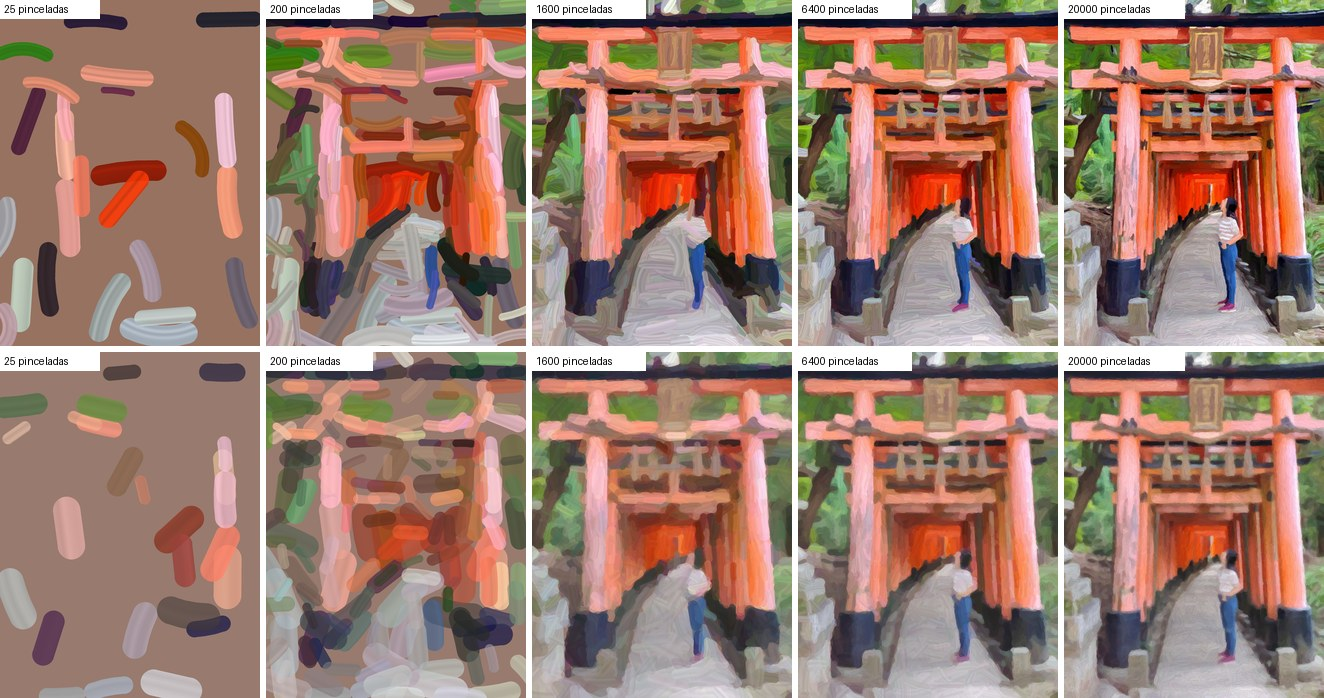
\includegraphics[width=\linewidth]{figuras/progreso.jpg}
\vspace{-0.5cm}
\caption{Capturas del lienzo durante la evolución (arriba: Van Gogh; abajo: Monet).}
\label{fig:progreso}
\end{figure}

\begin{figure}[t]
\centering
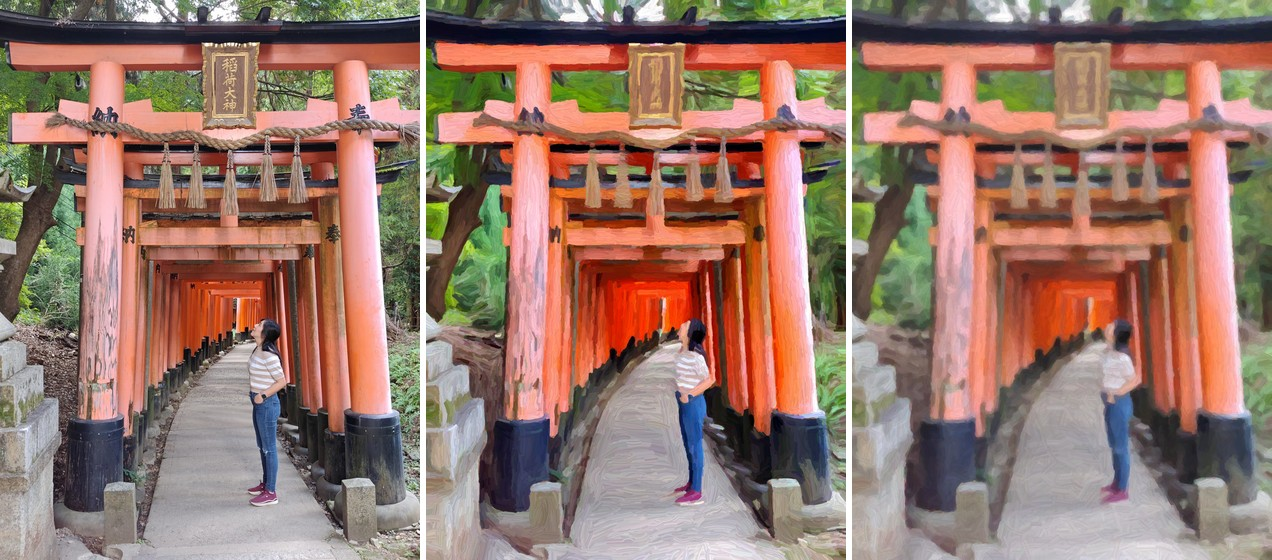
\includegraphics[width=0.92\linewidth]{figuras/final.jpg}
\vspace{-0.2cm}
\caption{Fotografía de entrada, resultado estilo Van Gogh y resultado estilo Monet (20{,}000 pinceladas cada uno, salida de $1200\times1600$\,px).}
\label{fig:final}
\end{figure}

\begin{figure}[t]
\centering
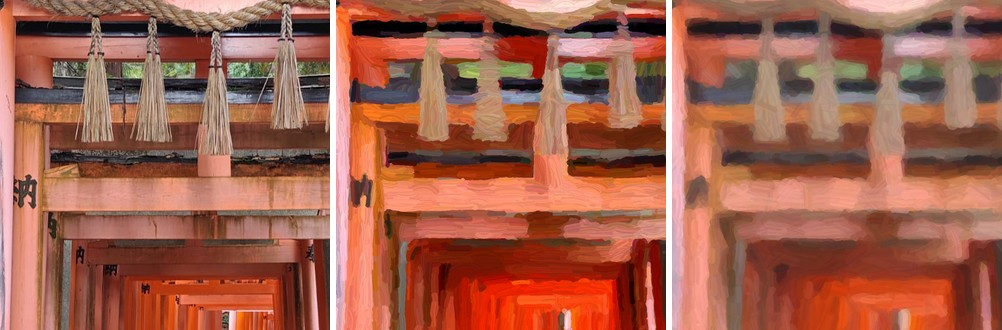
\includegraphics[width=0.8\linewidth]{figuras/detalle.jpg}
\vspace{-0.2cm}
\caption{Acercamiento a la misma zona: foto, Van Gogh (trazos largos y curvos con textura de cerdas) y Monet (toques cortos y semitransparentes).}
\label{fig:detalle}
\end{figure}

\begin{figure}[t]
\centering
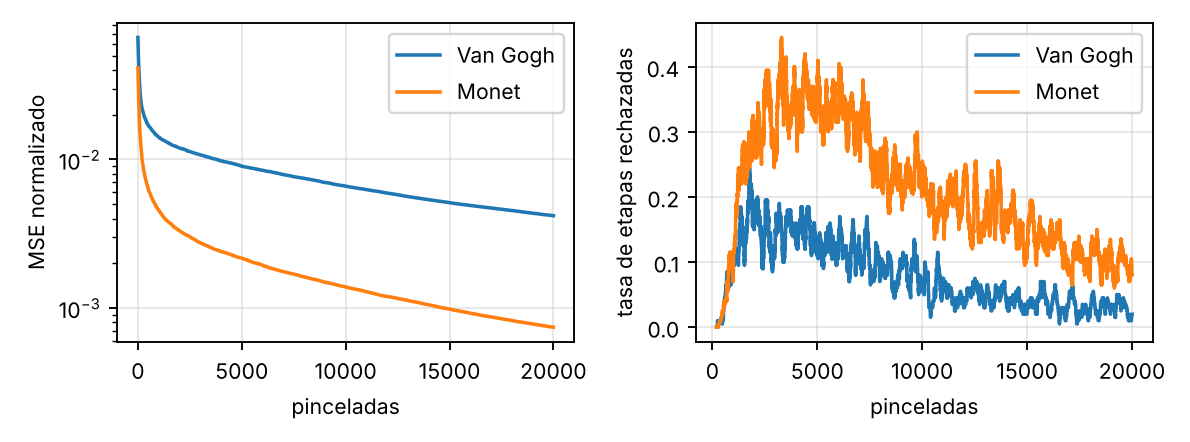
\includegraphics[width=0.85\linewidth]{figuras/convergencia_final.png}
\vspace{-0.3cm}
\caption{Corridas finales: MSE contra pinceladas (izq.) y tasa de etapas rechazadas, con media móvil de 200 etapas (der.).}
\label{fig:conv}
\end{figure}

\textbf{E1: ¿aporta la evolución?} La inicialización guiada ya es fuerte, así que es necesario comprobar que la selección, la cruza y la mutación agregan algo. Se comparó el AG contra una \emph{búsqueda aleatoria guiada}, que en cada etapa genera $16\times13=208$ pinceladas con la misma inicialización y conserva la mejor. Así ambos métodos usan exactamente el mismo número de evaluaciones. Se usó el estilo \emph{libre} (solo MSE), $300\times400$\,px, 3000 pinceladas y 3 semillas (Cuadro~\ref{tab:e1}, Fig.~\ref{fig:e1}). El AG reduce el MSE un \mejora\,\% de forma consistente: las desviaciones estándar son dos órdenes de magnitud menores que la diferencia. En el ajuste preliminar, la ventaja desapareció con pocas generaciones por etapa (8 individuos $\times$ 9 evaluaciones) y apareció al aumentarlas, lo que es coherente con que la explotación de la cruza y la mutación necesita varias generaciones. Como el AG tarda más por la sobrecarga de los operadores en Python, también se probó la búsqueda aleatoria con 273 evaluaciones por etapa, para un tiempo comparable (E1b). El AG sigue siendo mejor.

\begin{table}[h]
\centering\small
\caption{E1: AG contra búsqueda aleatoria guiada (media $\pm$ d.e., 3 semillas; 3000 pinceladas).}
\label{tab:e1}
\begin{tabular}{lccccc}
\toprule
Método & Evaluaciones & MSE & PSNR (dB) & SSIM & $t$ (s)\\
\midrule
AG (torneo, BLX-$\alpha$, mutación, elitismo) & \agEval\,mil & $\mathbf{\agMSE\pm\agSD}$ & \textbf{\agPSNR} & \textbf{\agSSIM} & \agT\\
Aleatoria guiada, mismas evaluaciones & \alEval\,mil & $\alMSE\pm\alSD$ & \alPSNR & \alSSIM & \alT\\
Aleatoria guiada, mismo tiempo (E1b) & \ebEval\,mil & \ebMSE & \ebPSNR & \ebSSIM & \ebT\\
\bottomrule
\end{tabular}
\end{table}

\begin{figure}[t]
\centering
\begin{minipage}{0.42\linewidth}
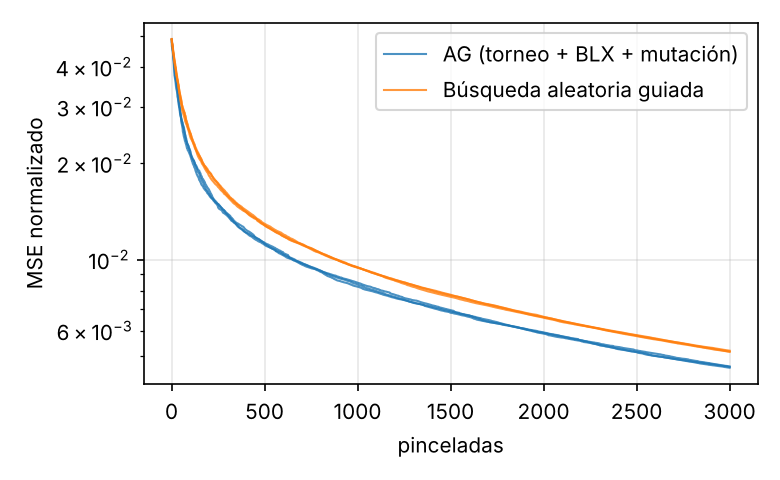
\includegraphics[width=\linewidth]{figuras/convergencia_ag_vs_aleatoria.png}
\vspace{-0.6cm}
\caption{E1: convergencia del AG frente a la búsqueda aleatoria guiada (3 semillas cada uno).}
\label{fig:e1}
\end{minipage}\hfill
\begin{minipage}{0.55\linewidth}
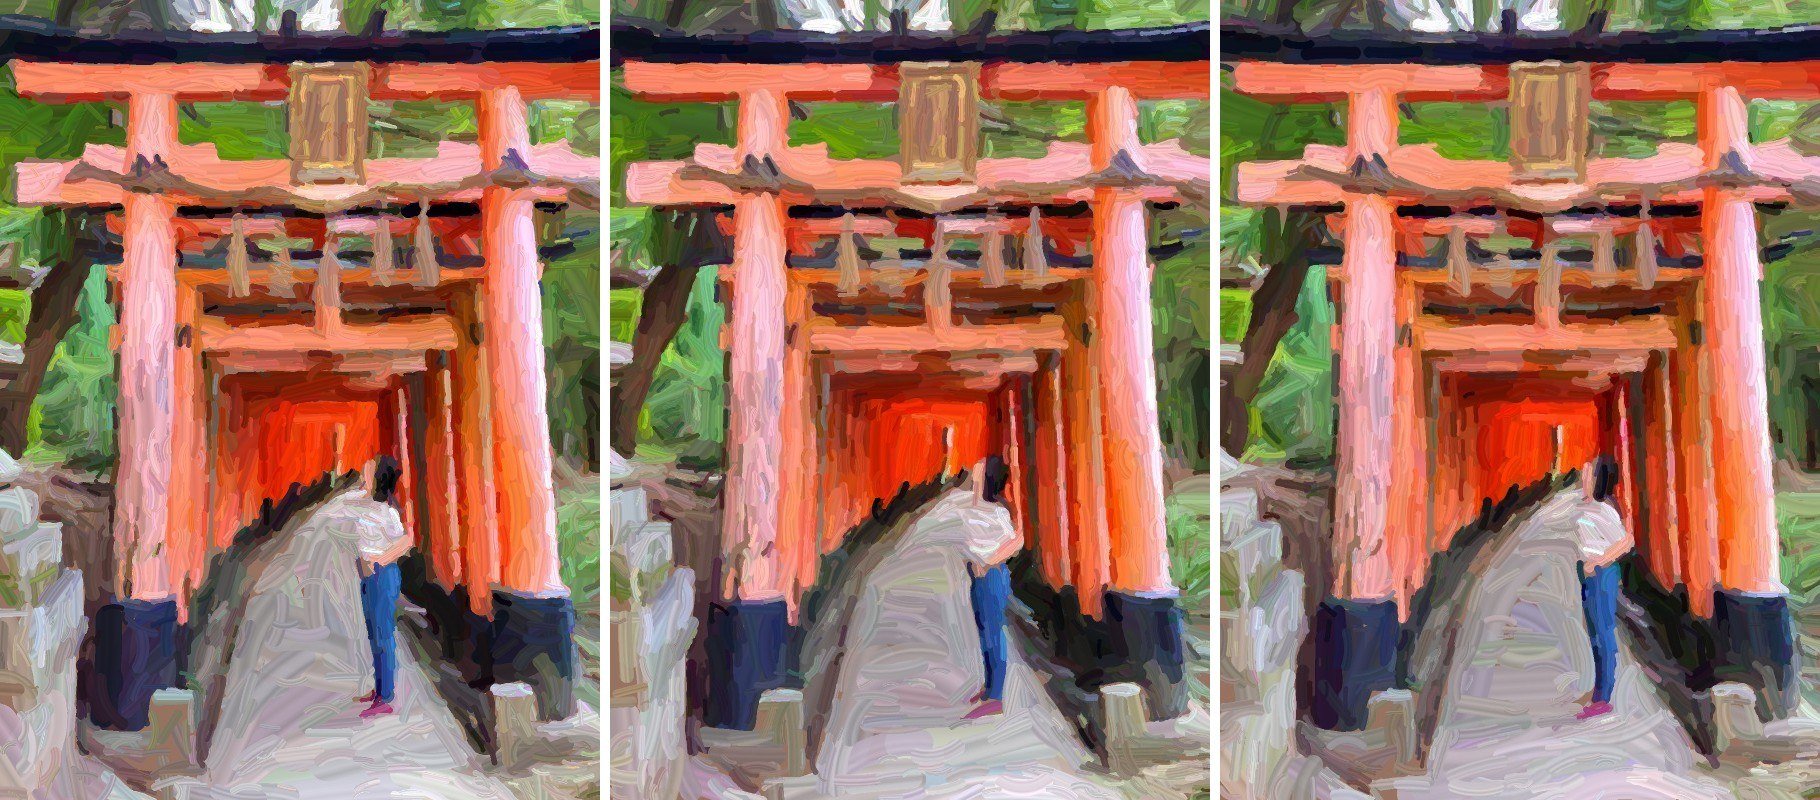
\includegraphics[width=\linewidth]{figuras/panel_lambda_flujo.jpg}
\vspace{-0.6cm}
\caption{E2: Van Gogh con $\lambda_\phi=0$, $0.04$ y $0.15$ (de izquierda a derecha).}
\label{fig:e2}
\end{minipage}
\vspace{-0.3cm}
\end{figure}

\textbf{E2: término de flujo.} Con el estilo Van Gogh y $\lambda_\phi\in\{0, 0.04, 0.15\}$, la desalineación media ponderada $\overline{\sin^2(\theta-\phi)}$ fue \lamCeroDes, \lamMedDes\ y \lamAltoDes, y el MSE fue \lamCeroMSE, \lamMedMSE\ y \lamAltoMSE. El término cumple su función: obliga a que los trazos sigan las formas (Fig.~\ref{fig:e2}) a cambio de un pequeño aumento del error. Es el compromiso explícito entre \emph{fidelidad} y \emph{estilo} de la Ec.~\ref{eq:fitness}.

\textbf{E3: tamaño del cromosoma.} Con $K=3$ pinceladas por individuo, el MSE con 3000 pinceladas fue \kTresMSE\ (\kTresT\,s), contra \kUnoMSE\ (\kUnoT\,s) con $K=1$. Al evolucionar varias pinceladas juntas, una buena queda ligada a otras malas y cada pincelada recibe menos evaluaciones. Por eso se eligió $K=1$.

% ==================================================================
\section{Discusión}
\textbf{Alcances.} El método reproduce imágenes arbitrarias con una estética pictórica reconocible. Los estilos se definen con un diccionario de parámetros, así que agregar otro pintor no requiere cambiar el algoritmo. El resultado se puede volver a dibujar a cualquier resolución, la corrida se puede interrumpir y reanudar, y el notebook ejecuta exactamente el mismo código que el script.

\textbf{Limitaciones.} (i) La descomposición secuencial es \emph{voraz}: una pincelada ya pintada no se vuelve a optimizar, así que el óptimo encontrado es local respecto al problema global. (ii) El ``estilo'' se impone con reglas (forma, objetivo estilizado y flujo), no se aprende de las pinturas reales. No hay una métrica objetiva de qué tan ``Van Gogh'' es el resultado, y la evaluación del estilo es cualitativa. (iii) La aptitud es el MSE en RGB, que no es perceptual; métricas como SSIM o el espacio Lab serían más fieles a la percepción humana. (iv) El costo es lineal en el número de pinceladas, del orden de $10^7$ evaluaciones para un resultado de alta calidad, y está limitado por la sobrecarga de Python. (v) Los parámetros del AG ($P$, $G$, $\sigma_0$) se ajustaron con una sola imagen.

\textbf{Trabajo futuro.} Comparar con estrategias evolutivas autoadaptativas (ES), re-optimizar las pinceladas ya colocadas, usar aptitud perceptual o de transferencia de estilo con una pintura de referencia, restringir los colores a la paleta del pintor y paralelizar la evaluación de la población.

% ==================================================================
\section{Conclusiones}
Se construyó un AG de codificación real que replica una imagen con pinceladas al estilo de Van Gogh y de Monet. Descomponer un problema de $2\times10^5$ variables en una secuencia de subproblemas de 10 variables, junto con la evaluación incremental y la inicialización guiada por el error, lo vuelve resoluble en minutos en una laptop. Con el mismo presupuesto de evaluaciones, los operadores evolutivos (torneo, BLX-$\alpha$, mutación gaussiana y elitismo) superan a la búsqueda aleatoria guiada. El término de flujo en la aptitud permite controlar el compromiso entre fidelidad y estilo.

\begin{thebibliography}{9}\small
\setlength\itemsep{0em}
\bibitem{engelbrecht} A.~P. Engelbrecht, \emph{Computational Intelligence: An Introduction}, 2.ª ed. Chichester: Wiley, 2007. Caps.~8--9.
\bibitem{blx} L.~J. Eshelman y J.~D. Schaffer, ``Real-coded genetic algorithms and interval-schemata,'' en \emph{Foundations of Genetic Algorithms 2}, pp.~187--202, 1993.
\bibitem{haeberli} P.~Haeberli, ``Paint by numbers: abstract image representations,'' \emph{SIGGRAPH Comput. Graph.}, 24(4):207--214, 1990.
\bibitem{hertzmann} A.~Hertzmann, ``Painterly rendering with curved brush strokes of multiple sizes,'' en \emph{Proc. SIGGRAPH}, pp.~453--460, 1998.
\bibitem{ssim} Z.~Wang, A.~C. Bovik, H.~R. Sheikh y E.~P. Simoncelli, ``Image quality assessment: from error visibility to structural similarity,'' \emph{IEEE Trans. Image Process.}, 13(4):600--612, 2004.
\end{thebibliography}

\end{document}
